\documentclass[a4paper,11pt]{article}

\usepackage[utf8]{inputenc}
%\usepackage[francais]{babel}
\usepackage[pdftex]{graphicx}
\usepackage{makeidx}
\makeindex
%\usepackage{url}
%\usepackage{hyperref} % make them clickable instead of url
\usepackage[pdftex,
            pdfauthor={Jan Krause},
            pdftitle={Data Repositories},
            pdfsubject={Repositories for research data publication},
            pdfkeywords={Data, Repository, Repositories, RDM, DMP, data lifecycle},
            pdfproducer={Latex},
            pdfcreator={pdflatex}]{hyperref}
\usepackage[pdftex]{graphicx}
\usepackage{array}
\usepackage{longtable}

\usepackage[backend=bibtex, sorting=nyt]{biblatex}
\addbibresource[label=mainbib]{./bibliography/RDMtools.bib}
%\usepackage{multirow}

\begin{document}

\begin{titlepage}

\begin{center}
\begin{minipage}[!t]{0.66\textwidth}
\begin{center}
    
\includegraphics[width=0.45\textwidth]{./images/epfl_logo.png}
    %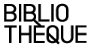
\includegraphics[width=0.45\textwidth]{./images/image_bibliotheque_small.png}  \\
    
\includegraphics[width=0.45\textwidth]{./images/logo_biblio.png}  \\
    %\textsc{École Poltechnique Fédérale de Lausanne} \\
    %\textsc{Bibliothèque}
    %\vspace{0.5cm}
\end{center}
\end{minipage}
\end{center}
%\hspace{4.3cm}
% \begin{minipage}[!t]{0.33\textwidth}
% \begin{flushright} \large
%     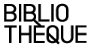
\includegraphics[width=0.70\textwidth]{./images/image_bibliotheque_small.png} \\
%     %\textsc{\Large Bibliothèque}  \\
%     %Jan \textsc{Krause} \\
% \end{flushright}
% \end{minipage}


\begin{center}

% Title

%\HRule \\[0.4cm]
\hrule

\vspace{3cm}

{ \huge \bfseries Data Repositories : \\ a publication guide}

%\HRule \\[1.5cm]

% Author and supervisor
%\begin{minipage}{0.4\textwidth}
%\begin{flushleft} \large
%\emph{Author:}\\
%\end{flushleft}
%\end{minipage}

%\begin{minipage}{0.4\textwidth}
%\begin{flushright} \large

\vspace{3cm}


by\\
\vspace{1.0cm}
{\Large Jan \textsc{Krause}} 
%\end{flushright}
%\end{minipage}

\vfill

% Bottom of the page
{\large \today}


\includegraphics{./images/CC-By-SA_88x31.png}

\end{center}

\end{titlepage}

\tableofcontents

\newpage
\section{Abstract}
\noindent This document is a \textbf{guide to data repositories for publication purposes}. It offers specific information for EPFL researchers.

\vspace{0.4cm}

\noindent Some sections of this this document were reproduced or adapted from ``\href{http://infoscience.epfl.ch/record/211157}{A Selection of Research Data Management Tools Throughout the Data Lifecycle}'' \cite{krause_selection_2015}, which adopts a more generalist point of view on research data management tools.


%\newpage
\section{Publishing your data}

Setting up a data management plan (DMP) is a way to covers prepare for all the issues related to a project data lifecycle management. At EPFL, you can get support at \href{mailto:datamanagementplan@epfl.ch}{datamanagementplan@epfl.ch}. Regarding data publication specifically, the following elements are of importance:
\begin{itemize}
\item \textbf{data format:} see section \ref{data_formats},
\item \textbf{metadata format:} see section \ref{metadata_formats},
\item \textbf{data licence:} see section \ref{data_licences},
\item \textbf{data workflow:} see section \ref{data_workflows}.
\end{itemize}

For working data or unpublished data \textbf{EPFL offers institutional storage \ref{epfl_storage}}.

\textbf{Domain repositories are generally recommended} because they offer adapted functionality (e.g. specific data and metadata adaptations) and are well know by the related community, thus maximiziong content's discoverability and reuse. To find a domain specific repository, \textbf{see section \ref{repositories_directories}}. In addition, a way to increase your datasets' impact are their description in data papers, see section \ref{data_papers}.

However, \textbf{all repositories are not to be trusted}: some might not last in long or even the mid term, be technically unreliable (broken links, bit rot...), and so on. For more information on the elements to \textbf{evaluate a repository trustworthiness, see section \ref{sigeldatpub}}.

Is no suitable domain data repositories is appropriated for a specific datastet, \textbf{generalist data repositories are available, see section \ref{repositories_generalist}}. Another option, may be to fall back on an institutional repository. Today, there is no such tool at EPFL, but \href{http://infoscience.epfl.ch}{Infoscience} may be used to publish small datasets. 

\section{Data repositories and storage}

The goal of this section is to help find a repository to publish datasets:
\begin{itemize}
\item \textbf{Generalist data repositories:} publish any type of data.
\item \textbf{Data repositories directories:} find the most appropriated repository for a specific dataset.
\item \textbf{Data papers and data journal:} data papers are publications describing datasets, which may be published in a repository or in a journal as supplementary material.
\item \textbf{Data storage at EPFL:} institutional storage infrastructures and related pricing.
\end{itemize}

In addition, in the next section (section \ref{sigeldatpub}, on page \pageref{sigeldatpub}) significant elements to consider for datasets publications are discussed.

\subsection{Generalist data repositories}
\label{repositories_generalist}

\noindent \index{Data Repositories!Zenodo} \textsc{\href{http://zenodo.org}{Zenodo}} \cite{zenodo_zenodo_2015}, \index{Data Repositories!Dryad} \textsc{\href{http://datadryad.org/}{dryad}} \cite{dryad_dryad_2015}  and \index{Data Repositories!Figshare} \textsc{\href{http://figshare.com/}{figshare}} \cite{figshare_figshare_2015} are state of the art general-purpose data repositories. Zenodo is made available by Cern and OpenAire and is free for any researcher publishing his or her data openly. Dryad is a curated repository, maintained by a non profit organization. Figshare belongs to a for profit company, the MacMillan group, which also owns the Nature Publishing Group.

\subsection{Data repositories directories}
\label{repositories_directories}

\noindent \index{Data Repositories!Re3data} \textsc{\href{http://re3data.org}{re3data.org}} is a registry of data repositories. This tool indexes over a thousand archives which are both subject specific and generalist and can be browsed by disciplines, available repositories features such as persistent identifiers support (e.g. DOIs, which play a crucial for guarantying access to datasets, as web links tend to break after a few years), and other important information such as data licenses availability, standards and policies \cite{re3data_re3data.org_2015}.

\vspace{0.4cm}

\noindent \index{Recommended!Data Repositories} \index{Data Repositories!Recommended Repositories} \textsc{\href{http://www.nature.com/sdata/data-policies/repositories}{Nature's Recommended Data Repositories}} is a set of disciplinary repositories covering the following fields: Biological sciences; Health sciences; Chemistry; Earth and environmental sciences; Physics, astrophysics \& astronomy; Social sciences; and General science \cite{nature_publishing_group_recommended_2014}.

\subsection{Data papers and data journals}
\label{data_papers}

\index{Data Journals!Data Papers} Data papers are publications describing datasets. In other words, they constitute peer-reviewed searchable metadata, and they can be used to find or highlight datasets. Data papers can be found in pure data journals, or in journals mixed with traditional scholarly publications. An important point, is that these papers may be found through classical scholarly search engines. In addition, the following resources can help you find multi-disciplinary datajournals and data papers:
\begin{itemize}
\item \index{Data Journals!Dryad's Data Journals List} \href{http://wiki.datadryad.org/Journal_instructions#Examples_of_journal_data_policies}{Dryad's examples of journal data policies} lists journals that require data archiving and journals with data policies \cite{dryad_journal_2015}
\item \index{Data Journals!Trac's atadData Journals List} Trac's multidisciplinary \href{http://proj.badc.rl.ac.uk/preparde/blog/DataJournalsList}{data journals list}\cite{trac_blog:_2013}
\item \index{Data Journals!Nature's Scientific Data} Nature Publishing Group's \href{http://www.nature.com/sdata/}{scientific data website} \cite{nature_publishing_group_scientific_2015}
\item DataShare's \href{https://www.wiki.ed.ac.uk/display/datashare/Sources+of+dataset+peer+review}{sources of dataset peer review} list of data journals \cite{datashare_sources_2015}
\item \index{Data Journals!GigaScience} \href{http://www.gigasciencejournal.com/}{GigaScience} \cite{gigascience_gigascience_2015}
\end{itemize}

Some discipline specific data journals exist too, for example:
\begin{itemize}
\item \index{Data Journals!Earth System Sicience Data} \index{Data Journals!Geoscience Data Journal} Wiley's \href{http://onlinelibrary.wiley.com/journal/10.1002/%28ISSN%292049-6060}{Geoscience Data Journal} and \href{http://www.earth-system-science-data.net/}{Earth System Science Data} \cite{earth_system_science_data_essd_2015}
\item \index{Data Journals!Open Health Data} UpMetaJournal's \href{http://openhealthdata.metajnl.com/}{Open Health Data} \cite{upmetajournals_open_2015}
\item \index{Data Journals!Biodiversity Data Journal} Pensoft's \href{http://biodiversitydatajournal.com/}{Biodiversity Data Journal} \cite{pensoft_biodiversity_2015}
\item \index{Data Journals!Archaeology Data Journal} UpMetaJournal's \href{http://openarchaeologydata.metajnl.com/}{Journal of open archaeology data} \cite{upmetajournals_journal_2015}
\end{itemize}

\noindent In addition, a list of \textsc{\href{http://datadryad.org/pages/jdap}{Journals Data Policies}} compiled by Dryad may be of interest \cite{dryad_joint_2014}.

\subsection{Data storage at EPFL}
\label{epfl_storage}

EPFL offers three types of storage\index{EPFL!Storage}, according to the \href{http://mediacom.epfl.ch/files/content/sites/mediacom/files/Flash/Flash%2004-2015.pdf}{Flash magazine, Number 4, 2015}:
\begin{itemize}
\item \textbf{Collaborative storage [Stockage collaboratif]:} The standard storage for lab. Each lab has by default 1TB offered, and may extend the capacity for 300CHF/TB/year. This service offers good performances and high resiliency (high ability to continue operating or recover if there is a failure). Indeed, data are replicated on a second geographical site and file history is preserved, allowing recovery after accidental modification or deletion. It may be used as a shared drive.
\item \textbf{On-line archive [Archive en ligne]:} This service is suited for data that are not modified frequently. It has the same degree of resiliency as the former service, but with lesser performances and version history. Its cost is of 200CHF/TB/year.
\item \textbf{Raw storage [Stockage brut]:} This storage may be viewed as a resilient virtual disk. It may be used as backup location for local data. The cost is of 100CHF/TB/year.
\end{itemize}

\noindent All the above storage solutions are located in Switzerland, and subject to Swiss law.

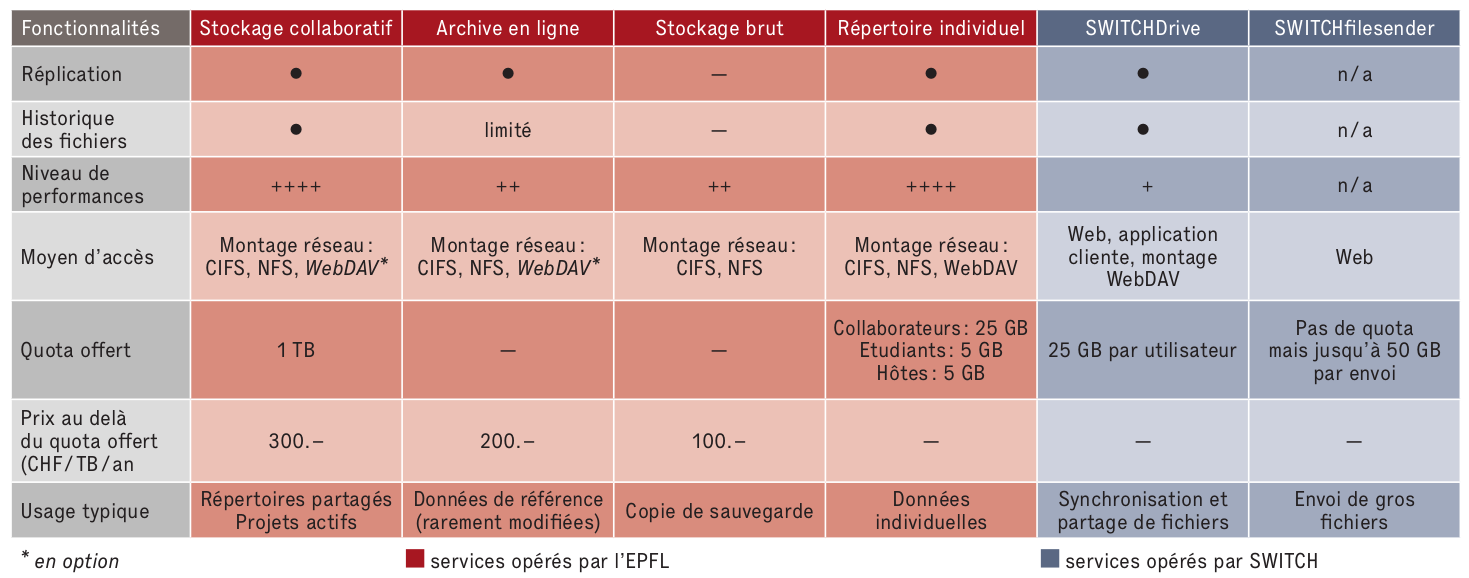
\includegraphics[width=1.0\textwidth]{./images/couts_stockage_flash.png}

Source: \href{http://mediacom.epfl.ch/files/content/sites/mediacom/files/Flash/Flash%2004-2015.pdf}{EPFL Flash, Number 4, 2015}.

\section{Significant elements for data publication}
\label{sigeldatpub}

The purpose of this section is to highlight and describe the diferent key elements to consider when publishing data.
\begin{itemize}
\item \textbf{Standards and certification:} Good practices ensure the visibility, accessibility, availability and integrity of datasets. They include attribution of persistent identifiers, data curation in general (such as bit preservation) and an appropriated infrastructure. Data repositories certifications guarantee a sufficient quality.
\item \textbf{Data formats:} The use of a standard data format increases datasets' interoperability. It is hence crucial to foster their reuse with other software or platforms, through time, and by other people as well.  
\item \textbf{Metadata Formats:} The use of a standard metadata format (or descriptive data) increases datasets' visibility in search engines, and the potential for their reuse.
\item \textbf{Data Worflows:} Reproducible research requires a good description of data provenance and computation workflow.
\item \textbf{Data and code licenses:} Licenses allow to define precisely what others may do with your data, and what they may not do.
\end{itemize}

In addition, in the next section (section \ref{sigeldatpub}, on page \pageref{sigeldatpub}) significant elements to consider for datasets publications are discussed.

\subsection{Standards and certifications}

\subsubsection{Peristant identifiers}

Persistent identifiers (PID) allow to identity unambiguously, resolve and retrieve datasets (and other digital objects). The most commonly used PIDs is the DOI (see below). PIDs avoid the loss of access to datasets due to broken links, which is quite frequent: A Plos One study showed in 2014 that more than 60\% of links to datasets are broken after 10
years \cite{pepe_how_2014}. Another Plos One 2014 article showed that the bibliography of one article out of five is impacted by that phenomenon \cite{van_de_sompel_scholarly_2014}.

\noindent The \index{Recommended!Digital Object Identifier (DOI)} \textsc{\href{http://www.doi.org/}{Digital Object Identifier (DOI)}} `` are characters strings (a "digital identifier") used to uniquely identify an object such as an electronic document. Metadata about the object is stored in association with the DOI name and this metadata may include a location, such as a URL, where the object can be found. The DOI for a document remains fixed over the lifetime of the document, whereas its location and other metadata may change. Referring to an online document by its DOI provides more stable linking than simply referring to it by its URL, because if its URL changes, the publisher need only update the metadata for the DOI to link to the new URL'' \cite{wikipedia_digital_2014}.

\subsubsection{Bit preservation}
Bitrot is a phenomenon more frequent than we think. Causes are complex and varied: disk errors, RAID errors, memory errors... \cite{harris_data_2007,panzer-steindel_data_2007}. To avoid this, some repositories offer bit preservation, or, even better are fully \href{http://public.ccsds.org/publications/archive/650x0m2.pdf}{OAIS} compliant \cite{wikipedia_oais_2015}.

\subsubsection{Certifications}
\noindent \index{Certifications!Data Seal of Approval} \textsc{\href{http://www.datasealofapproval.org/en/}{Data Seal of Approval}} and \noindent \index{Certifications!World Data System} \textsc{\href{http://www.icsu-wds.org/}{World Data System}} are the two main data repositories certifications. Certified repositories may be trusted, unfortunately only few repositories are certified at that time. 

\subsection{Data formats}
\label{data_formats}

\subsubsection{Generalist data formats}

\noindent \index{Recommended!HDF5} \index{Data Formats!HDF5} \textsc{\href{https://www.hdfgroup.org/HDF5/}{HDF5}} ``is a data model, library, and file format for storing and managing data. It supports an unlimited variety of datatypes, and is designed for flexible and efficient I/O and for high volume and complex data. HDF5 is portable and is extensible, allowing applications to evolve in their use of HDF5. The HDF5 Technology suite includes tools and applications for managing, manipulating, viewing, and analyzing data in the HDF5 format'' \cite{hdf_group_hdf5_2015}. HDF5 is supported form within many environments such as Matlab, Octave, Python (H5py, PyTables), GNU-R, Java, C++, Fortran and Mathematica.

\vspace{0.4cm}

\noindent The \index{Data Formats!Structured Query Language (SQL)} \textsc{\href{https://en.wikipedia.org/wiki/SQL}{Structured Query Language (SQL)}} ``a special-purpose programming language designed for managing data held in a relational database management system (RDBMS)''\cite{wikipedia_sql_2015}. SQL is well suited to store and share relational data. RDBMS are a great help in maintaining dateset's coherence and enforce data constraints. Several multi-platform open source RDBMS are available, such as \href{https://mariadb.org/}{MariaDB} (MySQL) \cite{mariadb_mariadb_2015} or \href{http://www.postgresql.org/}{PosgreSQL} \cite{postgresql_postgresql:_2015}.

\subsubsection{Subject specific data formats}

\noindent A directory of \index{Recommended!Data Formats} \index{Data Formats!Recommended Data Formats} \textsc{\href{http://www.digitalpreservation.gov/formats/}{Recommended Data Formats}} is maintained by the US Library of Congress. It covers the following categories: still images, sounds, moving images, textual documents, web archives, datasets, geospatial data as well as generic data \cite{libraryofcongress_sustainability_2015}.

\vspace{0.4cm}

\noindent The \index{Data Formats!Data Type Registry} \textsc{\href{http://www.typeregistry.org/registrar/}{DataTypeRegistry}} is a generic open source data type description platform. It allows in particular to combine already described units or data types to create new ones. Data types are labeled with unique identifiers. In addition to a web interface an automated access is allowed through the API \cite{datatyperegistry_data_2015}.

\subsection{Metadata formats}
\label{metadata_formats}

\subsubsection{Generalist metadata formats}
\noindent \index{Metadata Formats!DublinCore} \textsc{\href{http://dublincore.org/documents/dces/}{DublinCore}} is a vocabulary consisting of only 15 basic elements, such as Creator, Title, Date, Description, Format, Rights, or Subject \cite{dublincore_dublin_3013}. It is not specifically designed for dataset description, but widely used in scholarly communication. For that reason, it is a minimalist solution, and we recommend one of the solutions listed below instead. The basic DublinCore may be extended using \href{http://dublincore.org/documents/2000/07/11/dcmes-qualifiers/}{qualifiers}. 

\vspace{0.4cm}

\noindent \index{Metadata Formats!DataCite} \textsc{\href{https://schema.datacite.org/}{DataCite Metadata Schema}} is a standard designed with datasets in mind, and hence more adapted then DublinCore mentioned just above. For example, GeoLocation, ReserarchGroups, Collections, Videos or Workflows have their own specific resource types \cite{datacite_datacite_2015}.

\vspace{0.4cm}

\noindent Sometimes, a simple but clear \index{Metadata Formats!Textual description} \textsc{Textual Description} of a dataset can help a lot (even its own creator in the future). For instance, if it is not explicit in the dataset, it is a means to describe how, when, where and with what device the data has been gathered. In addition, the meaning of the labels (e.g. the column headers) are generally of interest, and so are the physical units and their accuracy.

\subsubsection{Subject specific metadata formats}

\noindent A directory of \index{Recommended!Metadata Formats} \index{Metadata Formats!Directory} \textsc{\href{http://rd-alliance.github.io/metadata-directory/}{Recommended Metadata Formats}} is available in this open source collaborative platform. They are indexed by discipline, extensions, associated tools and associated use cases. General available subject categories are Art and Humanities, Engineering, Life Sciences, Physical Sciences and Mathematics, Social and Behavioral Sciences and General Research Data. Dozens of subcategories are also available \cite{metadatadirectory_metadata_2015}.

\vspace{0.4cm}

\noindent The \index{Metadata Formats!Semantic Web (OWL)} \textsc{\href{http://www.w3.org/RDF/}{Semantic Web }} Resource Description Format (RDF) ``is a standard model data interchange on the Web''\cite{w3c_rdf_2014}. RDF is a very general format, however it my be used to describe precisely most types of data. Indeed, many \href{http://www.w3.org/2001/sw/wiki/OWL}{OWL} \cite{w3c_owl_2009} RDF based ontologies exist. Ontologies are ``formal naming and definition of types, properties and interrelationship'' of data \cite{wikipedia_ontology_2015}.

\subsubsection{Data and code licences}
\label{data_licences}

\noindent \index{Licences!Creative Commons By} \textsc{\href{https://creativecommons.org/}{Creative Commons BY}} licenses enable to choose exactly what is allowed to do with your datasets, text and multimedia documents. In addition to the CC0 (see below), the CC-BY offers 6 variants\cite{creativecommons.org_creative_2015}:
\begin{itemize}
\item
\includegraphics[width=15mm]{./images/CC-By_88x31.png} (Attribution : CC-By) ``lets others distribute, remix, tweak, and build upon your work, even commercially, as long as they credit you for the original creation. This is the most accommodating of licenses offered.''
\item
\includegraphics[width=15mm]{./images/CC-By-SA_88x31.png} (Attribution-ShareAlike) ``lets others remix, tweak, and build upon your work even for commercial purposes, as long as they credit you and license their new creations under the identical terms. [...] All new works based on yours will carry the same license, so any derivatives will also allow commercial use.''
\item
\includegraphics[width=15mm]{./images/CC-By-ND_88x31.png} (Attribution-NoDerivs) ``This license allows for redistribution, commercial and non-commercial, as long as it is passed along unchanged and in whole, with credit to you.''
\item
\includegraphics[width=15mm]{./images/CC-By-NC_88x31.png} (Attribution-NonCommercial) ``lets others remix, tweak, and build upon your work non-commercially, and although their new works must also acknowledge you and be non-commercial, they don’t have to license their derivative works on the same terms.''
\item
\includegraphics[width=15mm]{./images/CC-By-NC-SA_88x31.png} (Attribution-NonCommercial-ShareAlike) ``lets others remix, tweak, and build upon your work non-commercially, as long as they credit you and license their new creations under the identical terms.''
\item
\includegraphics[width=15mm]{./images/CC-By-NC-ND_88x31.png} (Attribution-NonCommercial-NoDerivs) ``This license is the most restrictive of [the Creative Commons] six main licenses, only allowing others to download your works and share them with others as long as they credit you, but they can’t change them in any way or use them commercially.''
\end{itemize}

\vspace{0.4cm}

\noindent \label{lcc0} \index{Licences!Creative Commons Zero} \textsc{\href{https://creativecommons.org/}{Creative Commons Zero}} 
\includegraphics[width=15mm]{./images/CC0-88x31.png}, contrarily to CC-By the ``CC0 enables scientists, educators, artists and other creators and owners of copyright- or database-protected content to waive those interests in their works and thereby place them as completely as possible in the public domain, so that others may freely build upon, enhance and reuse the works for any purposes without restriction under copyright or database law'' \cite{creativecommons.org_creative_2015}.

\noindent \index{Licences!GNU General Public Licence (GPL)} \textsc{\href{http://www.gnu.org/licenses/gpl.html}{GNU General Public licence (GPL)}} 
\includegraphics[width=15mm]{./images/gplv3-127x51.png} is to software what the Creative Commons Attribution-ShareAlike is to documents. It is the typical free software copyleft license and guarantees four freedoms to the users \cite{fsf_gpl_2105}:
\begin{itemize}
\item the freedom to use the software for any purpose,
\item the freedom to change the software to suit your needs,
\item the freedom to share the software with your friends and neighbors, and
\item the freedom to share the changes you make.
\end{itemize}

Many licences are compatible with GPLv3, notably: Apache Licence 2.0, Artistic Licence 2.0, Berkley Database Licence, Modified BSD License, Boost Software License, CeCILL, CreativeCommons Zero, Educationnal Community Licence, AGLP, LGPL, IBM Public Licence, Intel Open source License, ISC License, MIT License / X11 License, Python Software Lisence, W3C Software Notice and LicenseXFree86 Lisence, zlib/libpng License and Zope Public Lisence.  \cite{wikipedia_comparison_2015}

\vspace{0.4cm}

\noindent \index{Licences!GNU Lesser General Public Licence (LGPL)} \textsc{\href{http://www.gnu.org/licenses/lgpl.html}{GNU Lesser General Public licence (LGPL)}} ``The GNU Project has two principal licenses to use for libraries. One is the GNU Lesser GPL; the other is the ordinary GNU GPL. The choice of license makes a big difference: using the Lesser GPL permits use of the library in proprietary programs; using the ordinary GPL for a library makes it available only for free programs'' \cite{fsf_lgpl_2015}.

\vspace{0.4cm}

\noindent \index{Licences!GNU Affero General Public Licence (AGPL)} \textsc{\href{http://www.gnu.org/licenses/agpl.html}{GNU Affero Genreal Public licence (AGPL)}} ``The GNU Affero General Public License is a modified version of the ordinary GNU GPL version 3. It has one added requirement: if you run a modified program on a server and let other users communicate with it there, your server must also allow them to download the source code corresponding to the modified version running there. The purpose of the GNU Affero GPL is to prevent a problem that affects developers of free programs that are often used on servers'' \cite{fsf_agpl_2015}.

\subsubsection{Data Workflows}
\label{data_workflows}

\noindent \index{Software!MyExperiment} \textsc{\href{http://www.myexperiment.org}{myExperiment}} ``is a social website for sharing [...] scientific workflows [...]'' and integrates many tools such as Taverna and Bioclipse \cite{myexperiment_myexperiment_2014,myexperiment.org_myexperiment_2015}.

\vspace{0.4cm}

\noindent \index{Software!AiiDA} \index{EPFL!AiiDA} \textsc{\href{http://www.aiida.net/}{AiiDA}}, the Automated Interactive Infrastructure and Database for Computational is a ``flexible and scalable informatics' infrastructure to manage, preserve, and disseminate the simulations, data, and workflows of modern-day computational science. Able to store the full provenance of each object, and based on a tailored database built for efficient data mining of heterogeneous results, AiiDA gives the user the ability to interact seamlessly with any number of remote HPC resources and codes, thanks to its flexible plugin interface and workflow engine for the automation of complex sequences of simulations'' \cite{aiida.net_aiida_2015}. This tool is developed at EPFL. AiiDA's core is free software, some of its plugins are licensed for non-commercial use \cite{pizzi_aiida:_2015}.

\vspace{0.4cm}

\noindent \index{Software!Taverna} \index{Software!Pegasus} \textsc{\href{http://pegasus.isi.edu/}{Pegasus}} and \textsc{\href{http://www.taverna.org.uk/}{Taverna}} are open source workflow management systems, both able to execute applications \cite{pegasus_pegasus_2015,taverna_taverna_2015}.

\vspace{0.4cm}

\noindent \index{Software!Kepler} \textsc{\href{https://kepler-project.org/}{Kepler}} is a free software system for designing, executing, reusing, evolving, archiving, and sharing scientific workflows \cite{kepler-project.org_kepler_2015,kepler-project.org_kepler_2015-1}.

\vspace{0.4cm}

\noindent \index{Software!LIMS} \index{Software!SLIMS} \index{EPFL!SLIMS} \index{Software!OpenBIS} \textsc{\href{https://en.wikipedia.org/wiki/Laboratory_information_management_system}{Laboratory Information Management Systems}} are software that take modern laboratory operations in charge. Their features often include workflow management, data tracking, sample tracking, data exchange interfaces and enterprise resource planning \cite{wikipedia_laboratory_2015}. For example, at EPFL over 25 labs use the \href{http://sv-it.epfl.ch/slims}{SLIMS} software and ETHZ is developing an open source tool: \href{http://www.cisd.ethz.ch/software/openBIS}{openBIS} \cite{ethz_eth_2015,epfl_lsis_2015}.



\newpage
%\section{Index}
\printindex

\newpage
\printbibliography[title={Bibliography}]

\end{document}